% ==============================================================================
% 第 1 章：算术 (Chapter 1: Arithmetic)
% ==============================================================================

\chapter{算术}
\label{sec:ch01_arithmetic}

在序幕中，你已经学会了如何用初学学生语言（BSL）的记法来书写小学一年级就学过的算术表达式：
\begin{itemize}
  \item 写下左括号 \code{(}；
  \item 写下原生操作的名称 \code{op}；
  \item 写下操作的操作数（参数），各参数之间用空格分隔；
  \item 写下右括号 \code{)}。
\end{itemize}

作为回顾，这里给出一个最基本的原生表达式：
\begin{lstlisting}[language=BSL]
(+ 1 2)
\end{lstlisting}

它使用了加法操作符 \code{+} 来对两个数进行相加，其后跟着两个操作数，它们都是普通的数。但再看下面这个例子：
\begin{lstlisting}[language=BSL]
(+ 1 (+ 1 (+ 1 1) 2) 3 4 5)
\end{lstlisting}

第二个例子体现了上述语法规则中两个极其强大的特点：第一，原生操作可以接收两个以上的参数；第二，参数本身不一定必须是孤立的数值，它们也可以是嵌套的表达式。

\begin{notebox}[阅读建议]
快速浏览本章，直接跳到第~2~章；后续当你遇到不认识的“算术运算”时，再随时翻回本章查阅。
\end{notebox}

表达式的求值过程同样直截了当。首先，BSL 计算原生操作的所有参数表达式的值；其次，将计算得到的数据“喂给”该操作，由它计算出最终结果。因此：
\begin{lstlisting}[language=BSL]
(+ 1 2) == 3
\end{lstlisting}
以及：
\begin{lstlisting}[language=BSL]
(+ 1 (+ 1 (+ 1 1) 2) 3 (+ 2 2) 5)
== (+ 1 (+ 1 2 2) 3 4 5)
== (+ 1 5 3 4 5)
== 18
\end{lstlisting}

这些计算步骤对你来说应该十分熟悉，因为它们与你在数学课上所做的一模一样。你可能以前书写演算步骤的格式有所不同，或者从未系统学过如何一步步写下演算序列。但请放心，BSL 的计算法则与你从小掌握的算术完全一致，这足以令人心安。它保证了你能够清晰理解计算机对原生数据和原生操作做了什么，从而能够准确推导和预测程序的计算结果。一般而言，程序员必须深入透彻地理解编程语言的计算模型，否则程序的错误运算可能会危害到系统的使用者或其代表的利益。

\begin{notebox}[关于等号符号]
本书中使用记号 \code{==} 表示“根据计算法则两边完全等价”。
\end{notebox}

本章接下来的内容将介绍 BSL 的四种\term{原子数据}（atomic data）：数（Number）、字符串（String）、图像（Image）以及布尔值（Boolean）。我们借用了物理学中的“原子”概念：你无法窥探单个原子数据的内部构造，但可以通过函数将多个原子数据组合成新的数据，或者提取它们的属性（属性本身也是原子数据）等。本章各节将介绍处理这些数据的函数，它们通常被称为\term{原生操作}（primitive operations）或预定义操作。你也可以在 DrRacket 自带的 BSL 官方帮助文档中找到更多操作。

\begin{notebox}[进阶提示]
下一卷《How to Design Components》将深入解释如何自行设计原子数据。
\end{notebox}


% ==============================================================================
% 1.1 数的算术
% ==============================================================================
\section{数的算术}
\label{sec:1.1}

大多数人听到“算术”二字时，脑海中浮现的都是“数字”以及“对数字的操作”。“对数字的操作”意味着将两个数相加得到第三个数、从一个数中减去另一个数、计算两个数的最大公约数等等。如果我们不把算术限制得过于狭隘，它甚至可以包含计算角度的正弦值、将实数四舍五入为最接近的整数等数学运算。

BSL 语言原生支持数（Number）以及针对数的算术运算。正如序幕中所讨论的，加法等算术操作采用\term{前缀记法}（prefix notation）：
\begin{lstlisting}[language=BSL]
(+ 3 4)
\end{lstlisting}

语言为我们提供了非常丰富的数值操作：\code{+}、\code{-}、\code{*}、\code{/}、\code{abs}、\code{add1}、\code{ceiling}、\code{denominator}、\code{exact->inexact}、\code{expt}、\code{floor}、\code{gcd}、\code{log}、\code{max}、\code{numerator}、\code{quotient}、\code{random}、\code{remainder}、\code{sqr} 以及 \code{tan} 等等。我们只是按照字母顺序挑出了一些代表性的操作来展示其多样性。你可以在交互区中探索它们的用途，并去文档中看看还有哪些可用操作。

只要是你在数学课上学过的数值操作，BSL 大多都已经内置支持了。不妨猜猜它的函数名，并在交互区动手试一试。比如你需要计算某个角度的正弦值：
\begin{replbox}
> (sin 0)
0
\end{replbox}
你就可以放心使用它了。或者去查阅 DrRacket 的帮助手册（HelpDesk）。你会在手册中发现，除了丰富的数学函数外，BSL 还预定义了一些著名常数的名字，例如 \code{pi}（圆周率 $\pi$）和 \code{e}（自然常数 $e$）。

\begin{notebox}[常数 $e$（自然常数）]
你可能在微积分中接触过常数 $e$。它是一个实数，约等于 $2.718$，被称为“欧拉常数”或自然底数。
\end{notebox}

在数的种类上，BSL 程序可以使用自然数、整数、有理数、实数以及复数。我们假定你对除了复数之外的其他数都已相当熟悉。复数可能在高中数学课上提到过；如果没有也不必担心，虽然复数在科学计算中极其有用，但作为初学者完全无需掌握复数也能畅通无阻。

关于数值，一个极其关键的概念是\term{精度}（precision）。在现阶段，最重要的是理解 BSL 将数明确划分为\term{精确数}（exact numbers）与\term{不精确数}（inexact numbers）。在处理精确数时，BSL 尽可能全程保持完全精度。例如计算 \code{(/ 4 6)} 会产生精确的分数 \code{2/3}，DrRacket 可以将其呈现为真分数、假分数或混合小数。你可以用鼠标右键点击结果，在弹出菜单中切换分数的显示格式。

BSL 的某些数值操作无法产生精确结果。例如对 $2$ 使用 \code{sqrt}（开平方）操作，会产生一个无法用有限位数精确表示的无理数。由于计算机内存空间是有限的，BSL 必须将该数值适配到计算机中，因此会采用近似浮点数：\code{1.4142135623730951}。正如序幕中所提及的，前缀 \code{\#i} 会明确警示初学者该结果是不精确的。尽管绝大多数现代编程语言都通过降低精度来处理此类计算，但极少有语言能像 BSL 这样明确标注并主动提醒程序员。

\begin{notebox}[关于数的术语说明]
术语“数”（Number）指代了广泛的数值集合，包括计数、整数、有理数、实数乃至复数。在大多数日常场景中，你尽可以把 Number 等同于小学数轴上的数。当需要更加严谨时，我们会使用更精准的术语：Integer（整数）、Rational（有理数）等。甚至可以使用标准术语进行更细致的限定，如 PositiveInteger（正整数）、NonnegativeNumber（非负数）、NegativeNumber（负数）等。
\end{notebox}

\begin{exercise}{两点间距离计算}{1}
将以下针对 \code{x} 和 \code{y} 的定义添加到 DrRacket 的定义区：
\begin{lstlisting}[language=BSL]
(define x 3)
(define y 4)
\end{lstlisting}

现在将 \code{x} 和 \code{y} 想象为平面直角坐标系中一个点的横纵坐标。请写出一个表达式，计算该点到坐标原点 $(0,0)$ 的距离。

对于上述给定的初始值，预期的计算结果是 $5$。但你的表达式应当具备通用性：无论修改定义区中 \code{x} 和 \code{y} 的值为何，点击运行后都能正确计算出对应的距离。

如果你还没学过平面几何，或者忘记了相关公式，点 $(x,y)$ 到原点的欧几里得距离公式如下：
\[
  \sqrt{x^2 + y^2}
\]
毕竟我们的目标是教会你如何设计程序，而不是培养几何学家。

要构造这个表达式，最好的方法是点击【运行】（RUN）按钮并在交互区中进行交互式尝试。RUN 操作会让 DrRacket 获知 \code{x} 和 \code{y} 的当前值，这样你就能测试包含 \code{x} 和 \code{y} 的表达式：
\begin{replbox}
> x
3
> y
4
> (+ x 10)
13
> (* x y)
12
\end{replbox}

一旦在交互区找到了能得出正确结果的表达式，将其复制粘贴到定义区中。

为了检验表达式是否具有通用性，将定义区中的 \code{x} 修改为 \code{12}，\code{y} 修改为 \code{5}，再次点击【运行】，结果应当输出 \code{13}。
\end{exercise}

你的数学老师会说你刚刚计算了“距离公式”。为了在不同输入上复用该公式，你必须每次打开 DrRacket，编辑 \code{x} 和 \code{y} 的定义使其代表目标坐标，然后点击运行。但这种复用公式的方式既繁琐又笨拙。在第~2~章中，我们将很快为你介绍\term{函数}（function）的定义方法，它能让公式的复用变得极其优雅自然。目前安排此类练习，是为了引出函数思想，并为你即将开始的函数式编程做好铺垫。


% ==============================================================================
% 1.2 字符串的算术
% ==============================================================================
\section{字符串的算术}
\label{sec:1.2}

关于计算机内部运作，人们普遍存在一种偏见：许多人认为计算机内部全都是比特（bit）和字节（byte）——不论那到底是什么——并且充其量只能处理数字，因为人人都知道计算机会算术。诚然，电气工程师必须以这种方式理解和研究硬件，但初学者及其他任何应用开发者绝不需要（永远不需要）陷入这种底层思维。

编程语言的核心是处理\term{信息}（information），而现实世界的信息形态万千、各具特色。例如，程序可能需要处理颜色、人名、商务信函或人与人之间的对话。尽管我们理论上可以用一堆数字把所有信息都编码（例如规定 0 代表“红色”，1 代表“你好”），但这绝对是个糟糕至极的主意。试想一下，光是记忆庞大的对照表就会让人痛苦不堪。

因此，现代编程语言至少都会提供一种专门处理文本符号信息的数据类型。在 BSL 中，我们使用\term{字符串}（String）。通俗地说，字符串就是由双引号包围的字符序列，其中的字符可以通过键盘输入。在序幕中我们已经见过很多 BSL 字符串：\code{"hello"}、\code{"world"}、\code{"blue"}、\code{"red"} 等等。前两个是日常对话或信件中的词汇；后两个则是我们想要使用的颜色名称。

\begin{notebox}[关于 1String 的说明]
我们使用 \term{1String} 指代构成字符串的单个字符。例如，\code{"red"} 由三个 1String 构成：\code{"r"}、\code{"e"} 和 \code{"d"}。虽然在技术实现上 1String 有更完备的定义，但目前将其视为长度为 1 的字符串即可。
\end{notebox}

BSL 中只有一个专门接收字符串并产出字符串的原生操作：\code{string-append}。正如我们在序幕中所见，它将给定的多个字符串拼接为一个整体。可以将 \code{string-append} 理解为字符串世界的 \code{+}。加法接收两个（或更多）数字并产生一个新数字；拼接操作则接收两个（或更多）字符串并产生一个新字符串：
\begin{replbox}
> (string-append "what a " "lovely " "day" " 4 BSL")
"what a lovely day 4 BSL"
\end{replbox}

就像 \code{+} 相加时不会破坏或更改原有的数字一样，\code{string-append} 拼接时也绝不会篡改任何传入的字符串。要演算此类表达式，只需应用显而易见的运算法则即可：
\begin{center}
  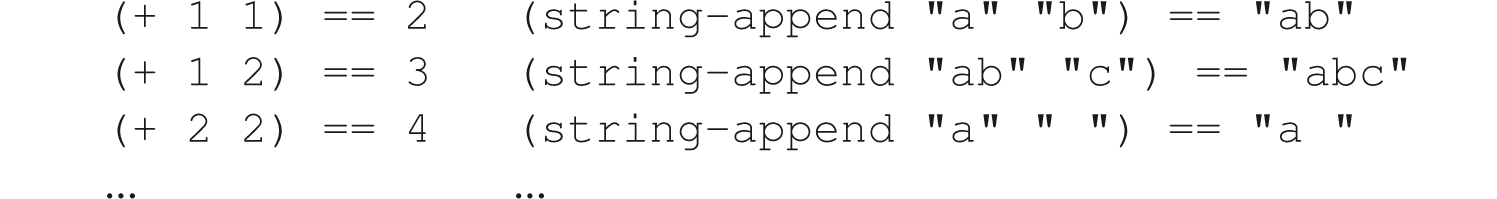
\includegraphics[width=0.7\textwidth]{images/00039.png}
\end{center}

\begin{exercise}{字符串拼接与连接符}{2}
在定义区添加以下两行代码：
\begin{lstlisting}[language=BSL]
(define prefix "hello")
(define suffix "world")
\end{lstlisting}

然后使用字符串原生操作编写一个表达式，将 \code{prefix} 与 \code{suffix} 拼接起来，并在两者中间插入下划线 \code{"\_"}。运行程序后，交互区应当输出 \code{"hello\_world"}。

参考练习~\ref{ex:1} 了解如何在 DrRacket 中测试与组织表达式。
\end{exercise}


% ==============================================================================
% 1.3 混合运算
% ==============================================================================
\section{混合运算}
\label{sec:1.3}

BSL 中所有其他与字符串相关的操作，要么接收非字符串数据，要么产生非字符串数据。以下是一些典型示例：
\begin{itemize}
  \item \code{string-length}：接收一个字符串，返回其字符个数（数）；
  \item \code{string-ith}：接收一个字符串 \code{s} 和一个整数 \code{i}，提取位于第 \code{i} 个位置的 1String（从 0 开始计数）；
  \item \code{number->string}：接收一个数，将其转换为对应的字符串。
\end{itemize}

请在帮助手册中查找并阅读 \code{substring} 的说明，了解它的具体功能。

如果文档中的描述一时难以理解，不妨直接在交互区中亲自实验这些函数。传入合适的参数观察其输出；也可以故意传入不合法的参数，看看 BSL 会如何报错：
\begin{replbox}
> (string-length 42)
string-length: expects a string, given 42
\end{replbox}

如你所见，BSL 会报告明确的错误信息。前半部分 \code{string-length} 指出哪个函数被误用了；后半部分则指明传入的参数错在何处。在这个例子中，\code{string-length} 期望接收一个字符串，但实际给入的却是一个数（即 42）。

当然，只要你清楚每个操作的输入输出类型，就可以自由地将处理不同类型数据的操作嵌套在一起。思考序幕中的这个表达式：
\begin{lstlisting}[language=BSL]
(+ (string-length "hello world") 20)
\end{lstlisting}

内层表达式对字符串 \code{"hello world"} 调用 \code{string-length}；外层表达式则让 \code{+} 将内层的结果与 \code{20} 相加。我们一步步推导该表达式的值：
\begin{lstlisting}[language=BSL]
(+ (string-length "hello world") 20)
== (+ 11 20)
== 31
\end{lstlisting}

不出所料，这种涉及不同数据类型的复合表达式的计算，与纯数值算术没有任何本质区别。再看另一个例子：
\begin{lstlisting}[language=BSL]
(+ (string-length (number->string 42)) 2)
== (+ (string-length "42") 2)
== (+ 2 2)
== 4
\end{lstlisting}

在继续学习之前，请尝试构造几个错误混合数据类型的嵌套表达式，例如：
\begin{lstlisting}[language=BSL]
(+ (string-length 42) 1)
\end{lstlisting}
在 DrRacket 中运行它们。仔细观察红色的错误提示信息，并注意观察定义区中被高亮标出的出错位置。

\begin{exercise}{在指定位置插入字符}{3}
在定义区添加以下两行：
\begin{lstlisting}[language=BSL]
(define str "helloworld")
(define i 5)
\end{lstlisting}

然后使用字符串原生函数编写一个表达式，在第 \code{i} 个位置插入下划线 \code{"\_"}。通常这意味着生成的新字符串会比原字符串更长；在当前测试中，预期结果为 \code{"hello\_world"}。

位置（position）表示从字符串最左端开始偏移的字符数，但程序员从 0 开始计数。因此在当前例子中，第 5 个字符是 \code{"w"}，因为第 0 个字符是 \code{"h"}。

\textbf{计数提示：}遇到此类索引计数问题时，可以在 \code{str} 下方添加一个数字索引字符串来辅助观察：
\begin{lstlisting}[language=BSL]
(define str "helloworld")
(define ind "0123456789")
(define i 5)
\end{lstlisting}
\end{exercise}

\begin{exercise}{删除指定位置的字符}{4}
沿用练习~\ref{ex:3} 中的相同设定，编写一个表达式，从字符串 \code{str} 中删除第 \code{i} 个位置的字符。显然，这个新字符串会比原字符串短一个字符。对于给定的字符串，\code{i} 取哪些值是合法且有效的？
\end{exercise}


% ==============================================================================
% 1.4 图像的算术
% ==============================================================================
\section{图像的算术}
\label{sec:1.4}

\term{图像}（Image）是一种可视化的二维矩形数据，例如照片、几何图形或绘图画布。在 DrRacket 中，凡是可以书写表达式的地方都可以直接插入图像，因为图像也是一等值（Value），与数和字符串处于同等地位。

\begin{notebox}[图像库引入]
在新的代码窗口中使用图像功能前，请务必在定义区顶部声明：\code{(require 2htdp/image)}。
\end{notebox}

你的程序可以通过原生操作来创建与变换图像。这些原生图像操作主要分为三大类。第一类用于创建基础图形：
\begin{itemize}
  \item \code{circle}：根据半径、填充模式和颜色创建圆形；
  \item \code{ellipse}：根据横向半径、纵向半径、填充模式和颜色创建椭圆；
  \item \code{line}：根据两点相对位移和颜色绘制线段；
  \item \code{rectangle}：根据宽度、高度、填充模式和颜色创建矩形；
  \item \code{text}：根据文本内容、字号和颜色渲染文本图像；
  \item \code{triangle}：根据边长、填充模式和颜色创建顶点向上的等边三角形。
\end{itemize}

这些操作的名称清晰指明了所创建图形的种类。你只需要知道，模式参数通常是 \code{"solid"}（实心）或 \code{"outline"}（轮廓线），而颜色参数是如 \code{"orange"}、\code{"black"} 等颜色名称字符串。

在交互区中实际尝试这些操作，如图~\ref{fig:ch01_image_intro} 所示：
\begin{figure}[htbp]
  \centering
  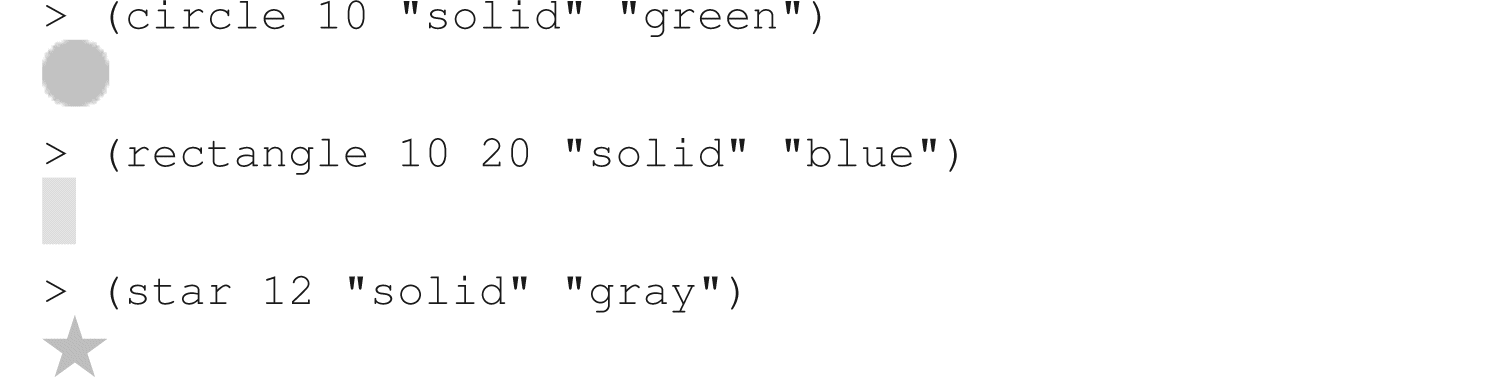
\includegraphics[width=0.75\textwidth]{images/00040.png}
  \caption{在交互区中测试基础图形创建操作}
  \label{fig:ch01_image_intro}
\end{figure}

请停下来思考！上面这段截图中出现了一个前文未提及的操作。请查阅帮助文档，看看 \code{2htdp/image} 库中还提供了哪些基础图形绘制函数，并亲自实验探索。

第二类图像函数用于测量图像属性：
\begin{itemize}
  \item \code{image-width}：以像素为单位获取图像的宽度；
  \item \code{image-height}：以像素为单位获取图像的高度。
\end{itemize}

它们能从图像中提取出符合直觉的数值：
\begin{replbox}
> (image-width (circle 10 "solid" "red"))
20
> (image-height (rectangle 10 20 "solid" "blue"))
20
\end{replbox}

请停下来思考！解释 DrRacket 是如何一步步求出以下表达式的值的：
\begin{lstlisting}[language=BSL]
(+ (image-width (circle 10 "solid" "red"))
   (image-height (rectangle 10 20 "solid" "blue")))
\end{lstlisting}

为了透彻理解第三类图像组合操作，需要引入一个新概念：\term{锚点}（anchor point）。图像不是孤立的单个像素，而是由许多像素构成的矩形区域。每个图像都像一张照片，其矩形范围内部有一个隐式的基准锚点。当你使用图像合成函数将两张图像叠合时，除非明确指定，否则默认都是围绕各自的锚点对齐的：
\begin{itemize}
  \item \code{overlay}：将传入的多个图像依次叠放在一起，默认以各自的中心点作为对齐锚点；
  \item \code{overlay/xy}：类似于 \code{overlay}，但在两个图像之间额外接收两个数值 \code{x} 和 \code{y}。它将第二张图像相对于第一张图像的左上角向右平移 \code{x} 像素，向下平移 \code{y} 像素；负的 \code{x} 向左移动，负的 \code{y} 向上移动；
  \item \code{overlay/align}：类似于 \code{overlay}，但接收两个字符串指定对齐边缘（例如 \code{"center"}、\code{"left"}、\code{"right"}、\code{"top"}、\code{"bottom"} 等），共有 9 种可能的对齐组合。
\end{itemize}

\code{2htdp/image} 库还包含了许多用于合成图像的高级函数。随着你逐步熟悉图像处理，可以进一步阅读文档。目前我们再介绍三个关键函数，它们对于构建游戏和交互动画至关重要：
\begin{itemize}
  \item \code{empty-scene}：创建指定宽度和高度的空白矩形画布（场景）；
  \item \code{place-image}：将一张图像放置在场景中的指定坐标位置。如果图像超出了画布边界，超出部分会被自动裁切；
  \item \code{scene+line}：接收一个场景、两点坐标数值和颜色，在场景上绘制一条直线。
\end{itemize}

图像算术的演算法则与数的算术完全类似；参见图~\ref{fig:ch01_image_laws} 中给出的示例及其与数值算术的对照。同样，任何原始图像都不会被修改或破坏，这些操作只是依据输入合成了全新的图像对象。

\begin{figure}[htbp]
  \centering
  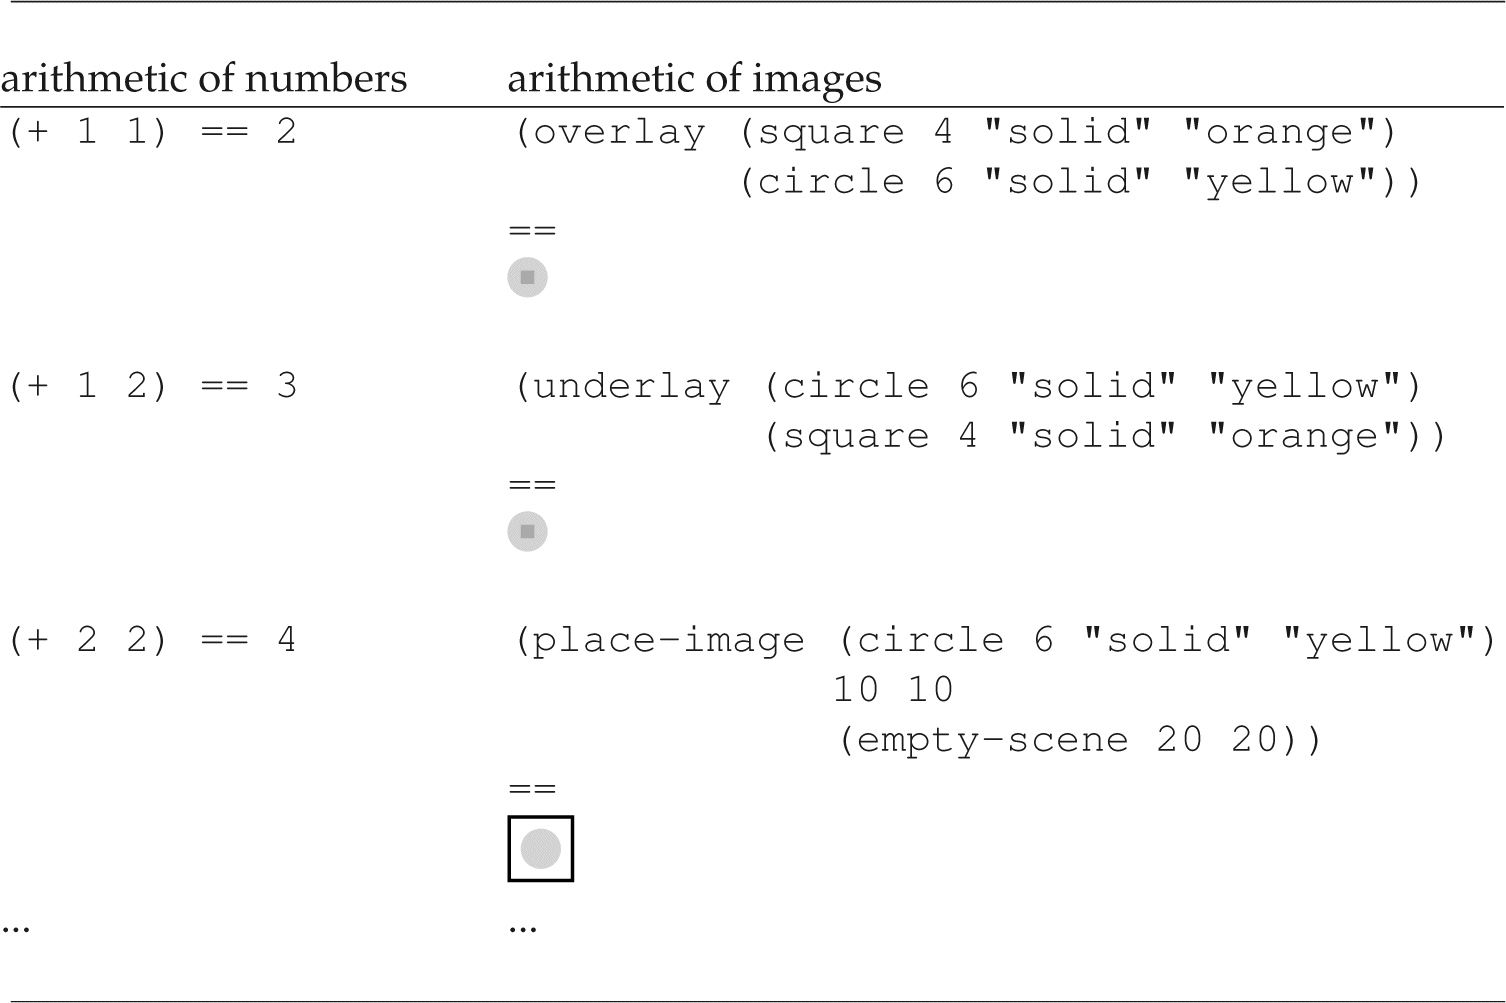
\includegraphics[width=0.85\textwidth]{images/00041.png}
  \caption{图像构造的代数演算法则与数值计算的类比}
  \label{fig:ch01_image_laws}
\end{figure}

\begin{exercise}{创建小船或小树图像}{5}
使用 \code{2htdp/image} 库中的绘图函数，拼装出一艘简易小船或一棵小树的图像。注意在设计代码时保持清晰结构，使得后续能够方便地通过修改参数来整体缩放图像大小。
\end{exercise}

\begin{exercise}{计算图像的像素数}{6}
在定义区添加以下代码：
\begin{center}
  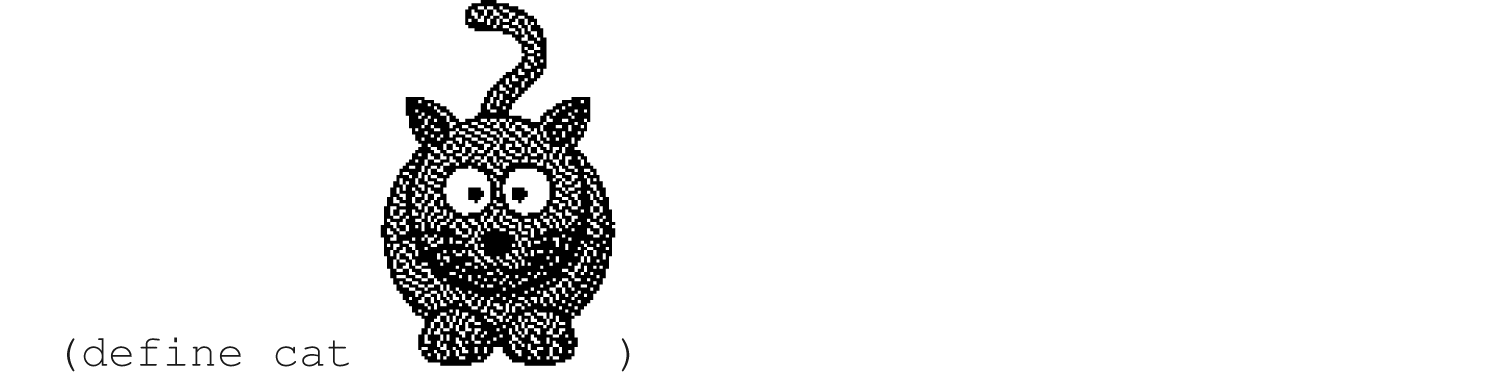
\includegraphics[width=0.55\textwidth]{images/00042.png}
\end{center}

\textbf{图片复制技巧：}你可以直接从电子书中复制该小猫图片，并直接粘贴到 DrRacket 的定义区代码中。

编写一个表达式，计算该图像所包含的总像素数（即像素面积）。
\end{exercise}


% ==============================================================================
% 1.5 布尔值的算术
% ==============================================================================
\section{布尔值的算术}
\label{sec:1.5}

在正式动手设计程序之前，我们还需要掌握最后一种基础原子数据：\term{布尔值}（Boolean values）。布尔值只有两个：\code{\#true} 和 \code{\#false}。在程序中，布尔值主要用来表示条件决策的结果或各种开关的状态。

布尔值的运算同样非常简单。BSL 程序主要使用三个逻辑操作：\code{or}（逻辑或）、\code{and}（逻辑与）和 \code{not}（逻辑非）。它们在逻辑世界中的角色，就像数的加法、乘法与取相反数。由于布尔值只有两种可能，我们可以穷举列出所有可能情况下的运算行为：
\begin{itemize}
  \item \code{or}：检查传入的布尔值中是否存在任意一个 \code{\#true}：
\begin{replbox}
> (or #true #true)
#true
> (or #true #false)
#true
> (or #false #true)
#true
> (or #false #false)
#false
\end{replbox}

  \item \code{and}：检查传入的布尔值是否全部都为 \code{\#true}：
\begin{replbox}
> (and #true #true)
#true
> (and #true #false)
#false
> (and #false #true)
#false
> (and #false #false)
#false
\end{replbox}

  \item \code{not}：逻辑取反，总是返回与给定布尔值相反的值：
\begin{replbox}
> (not #true)
#false
> (not #false)
#true
\end{replbox}
\end{itemize}

和加法类似，\code{or} 与 \code{and} 也可以接收两个以上的布尔表达式。另外，\code{or} 和 \code{and} 还有短路求值等更深刻的特性，这需要我们在更复杂的嵌套表达式中进一步探究。

\begin{exercise}{商场购物条件判断}{7}
布尔表达式能够精确描述许多日常生活中的决策逻辑。假设你想决定今天是否适合去商场逛街。你的决策准则是：只要“今天不是晴天”或者“今天是周五”（因为商场周五会推出全新打折特卖），你就去商场。

按照你刚刚学到的布尔运算知识，首先在 DrRacket 定义区添加以下两行：
\begin{lstlisting}[language=BSL]
(define sunny #true)
(define friday #false)
\end{lstlisting}

现在编写一个表达式，判断在“\code{sunny} 为假”或者“\code{friday} 为真”时是否前往商场。在当前的具体设定下，计算结果应当是 \code{\#false}（为什么？）。

请参考练习~\ref{ex:1} 组织测试。\code{sunny} 和 \code{friday} 两个变量一共有多少种不同的布尔值组合？
\end{exercise}


% ==============================================================================
% 1.6 布尔混合运算
% ==============================================================================
\section{布尔混合运算}
\label{sec:1.6}

布尔值的一大核心用途是与其他类型的数据协同进行条件计算。在序幕中我们知道，BSL 允许通过定义为数据命名。例如，我们可以用以下代码开始一个程序：
\begin{lstlisting}[language=BSL]
(define x 2)
\end{lstlisting}
然后计算其倒数：
\begin{lstlisting}[language=BSL]
(define inverse-of-x (/ 1 x))
\end{lstlisting}
这在平时运转良好，但如果我们把 \code{x} 的值修改为 \code{0}，程序就会因除以零而崩溃。

这就凸显了布尔值与条件分支的威力。首先，原生判断函数 \code{=} 用来判断两个（或多个）数是否相等。如果相等则返回 \code{\#true}，否则返回 \code{\#false}。其次，BSL 提供了条件分支形式：\term{\code{if} 表达式}。\code{if} 的用法看起来类似原生函数，但它实际上是核心语法形式。\code{if} 后面跟随三个子表达式，各部分以空格分隔，整体由括号包围：
\begin{lstlisting}[language=BSL]
(if (= x 0) 0 (/ 1 x))
\end{lstlisting}

该 \code{if} 表达式包含了三个子表达式：\code{(= x 0)}、\code{0} 以及 \code{(/ 1 x)}。\code{if} 表达式的求值严格遵循两步法则：
\begin{enumerate}
  \item 首先必定对第一个条件子表达式求值，其计算结果必须是一个布尔值（\code{\#true} 或 \code{\#false}）；
  \item 若条件为 \code{\#true}，则对第二个子表达式求值并将其作为整个 \code{if} 的结果；若条件为 \code{\#false}，则对第三个子表达式求值并作为结果。
\end{enumerate}

在给定 \code{x} 为 2 的定义下，你可以在交互区中试验该表达式：
\begin{replbox}
> (if (= x 0) 0 (/ 1 x))
0.5
\end{replbox}

根据代数计算法则，你可以自行手动推导其求值步骤：
\begin{lstlisting}[language=BSL]
(if (= x 0) 0 (/ 1 x))
== ; 因为全局变量 x 的当前值为 2
(if (= 2 0) 0 (/ 1 2))
== ; 2 不等于 0，(= 2 0) 计算结果为 #false
(if #false 0 (/ 1 2))
== ; if 分支依据 #false 选取第三个子表达式
(/ 1 2)
== ; 转换为十进制显示
0.5
\end{lstlisting}

换句话说，DrRacket 知道 \code{x} 代表 2 且不等于 0，因此 \code{(= x 0)} 得到 \code{\#false}，驱动 \code{if} 仅计算第三个子表达式 \code{(/ 1 x)}，完全避免了潜在的除以零错误！

请停下来思考！假设将定义区修改为：
\begin{lstlisting}[language=BSL]
(define x 0)
\end{lstlisting}
在此时的环境下，\code{(if (= x 0) 0 (/ 1 x))} 会计算出什么结果？为什么？请写出一步步的演算序列。

除 \code{=} 外，BSL 还提供了全套数值比较操作符：\code{<}（小于）、\code{<=}（小于等于）、\code{>}（大于）和 \code{>=}（大于等于）。请解释它们各自的判断规则。

注意：字符串不能使用 \code{=} 进行比较。如果需要比较字符串，必须使用专门的字符串比较操作符：\code{string=?}、\code{string<=?} 或 \code{string>=?}。\code{string=?} 显然是判断两个字符串内容是否完全一致，而后两者则是按字典序进行比较。你可以查阅文档并动手验证。

你可能会好奇，为什么程序需要比较字符串？想象一个控制红绿灯交通信号灯的程序，它可能使用字符串 \code{"green"}、\code{"yellow"} 和 \code{"red"} 来表示灯的颜色。程序中可能包含类似下面的片段：
\begin{lstlisting}[language=BSL]
(define current-color ...)
(define next-color
  (if (string=? "green" current-color) "yellow" ...))
\end{lstlisting}
显然，这段代码负责根据当前灯的颜色计算下一个应当点亮的状态。

在接下来的章节中，我们将介绍比简单的 \code{if} 更强大、更优雅的条件表达式（例如 \code{cond}），以及设计复杂条件分支的系统化方法。

\begin{exercise}{图像长宽比分类}{8}
在定义区添加以下代码：
\begin{center}
  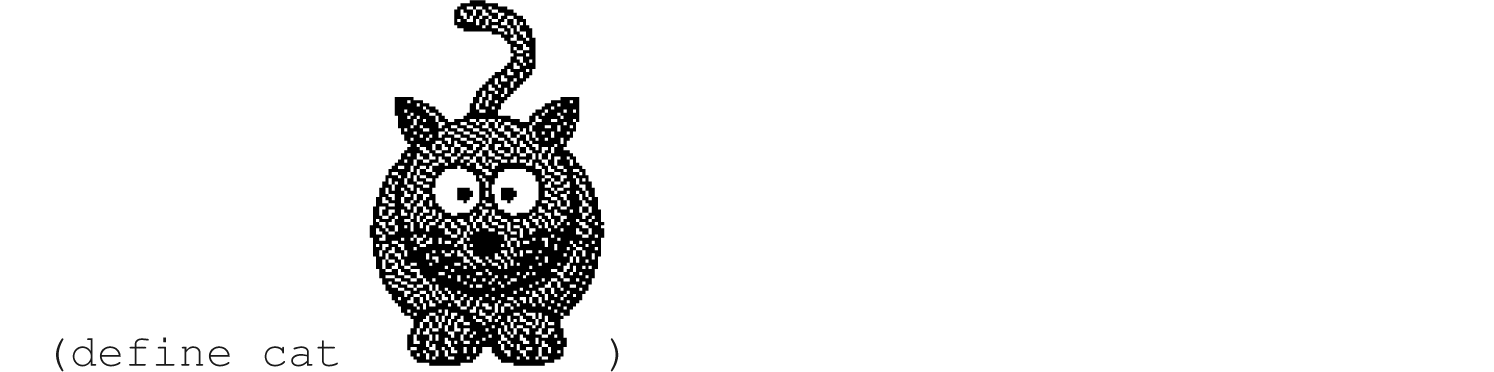
\includegraphics[width=0.55\textwidth]{images/00043.png}
\end{center}

编写一个条件表达式，判断该图像是瘦高形（\code{"tall"}）还是矮宽形（\code{"wide"}）。如果高度大于等于宽度，判定为 \code{"tall"}；否则判定为 \code{"wide"}。在测试时，可以把小猫图片临时替换为你自己创建的不同长宽的矩形，以确保能够预测并验证答案。

进一步拓展：修改你的条件表达式，让它能够将图像细分为三类：\code{"tall"}（高）、\code{"wide"}（宽）还是 \code{"square"}（正方形）。
\end{exercise}


% ==============================================================================
% 1.7 谓词：了解你的数据
% ==============================================================================
\section{谓词：了解你的数据}
\label{sec:1.7}

还记得前文中执行 \code{(string-length 42)} 时触发的错误吗？严格来说，这个表达式并没有产生任何值，而是直接中断并报错。DrRacket 在交互区用醒目的红色文字展示错误，并在定义区高亮标出出错代码。当错误深藏于长串嵌套表达式之中时，这种定位机制尤为有用：
\begin{lstlisting}[language=BSL]
(* (+ (string-length 42) 1) pi)
\end{lstlisting}
你可以在交互区和定义区分别输入此表达式并运行，体会错误高亮的效果。

在真正的实际程序中，你绝不希望出现此类未捕获的运行时崩溃。虽然你通常不会写出把字面量 \code{42} 当成字符串这样明显的低级错误，但在实际项目中，变量所绑定的数据类型往往存在不确定性：
\begin{lstlisting}[language=BSL]
(define in ...)
(string-length in)
\end{lstlisting}
变量 \code{in} 可能由外部输入提供，它既可能是一个字符串，也可能意外接收到了一个数。

防止这种崩溃的最佳手段是使用\term{谓词}（predicate）。谓词是一种特殊的函数，它接收一个任意值，并判断该值是否属于某一特定数据类型。例如谓词 \code{number?} 判断给定值是否为数值：
\begin{replbox}
> (number? 4)
#true
> (number? pi)
#true
> (number? #true)
#false
> (number? "fortytwo")
#false
\end{replbox}

如你所见，谓词总是返回布尔值。因此，将谓词与条件分支配合使用，就能构筑起坚固的数据防护栏，使程序免受类型错误的影响：
\begin{lstlisting}[language=BSL]
(define in ...)
(if (string? in) (string-length in) ...)
\end{lstlisting}

本章介绍的每一种数据类型都有其对应的内置谓词：\code{number?}、\code{string?}、\code{image?} 以及 \code{boolean?}。请在交互区中逐一尝试，确保完全理解其用法。

\begin{notebox}[有趣的复数探秘]
在交互区的提示符后输入 \code{(sqrt -1)} 并按下回车。仔细观察输出结果：你会看到类似 \code{0+1i} 的结果，这就是大家接触到的第一个复数。尽管中学数学老师可能说过“负数不能开平方”，但在高等数学与工程编程中，复数计算极其广泛且极其有用。不过不必担忧，理解复数并非成为优秀程序设计师的先决条件。
\end{notebox}

除了区分不同数据形态的基础谓词外，编程语言通常还提供用于细分数值子类型的谓词。在 BSL 中，数主要按两套维度分类：构造形式（construction）与精确度（exactness）。

按构造形式分类对应我们熟悉的数学数集：\code{integer?}（整数）、\code{rational?}（有理数）、\code{real?}（实数）和 \code{complex?}（复数）。不过由于包括 BSL 在内的很多编程语言在内部对某些著名数学常数采用有限精度近似表示，有时使用 \code{rational?} 会得到令人微感意外的判定：
\begin{replbox}
> (rational? pi)
#true
\end{replbox}
这是因为浮点近似值在计算机内部表示为二进制有理数。

关于精确度，我们在前文已有所涉猎。你可以使用 \code{exact?}（是否精确）和 \code{inexact?}（是否不精确）来进行检测。后续我们还会深入探讨数的本质特征。

\begin{exercise}{将任意数据转换为正数}{9}
在 DrRacket 定义区添加以下代码：
\begin{lstlisting}[language=BSL]
(define in ...)
\end{lstlisting}

编写一个综合条件表达式，将变量 \code{in} 所绑定的任意合法值转换为一个非负数：
\begin{itemize}
  \item 若为字符串，计算该字符串的长度；
  \item 若为图像，计算其像素面积（宽 $\times$ 高）；
  \item 若为数值，当该数大于 0 时将其减 1，若已经是 0 或负数则保持为该数或取 0；
  \item 若为布尔值，当为 \code{\#true} 时取 10，为 \code{\#false} 时取 20。
\end{itemize}
使用本节所学的各种类型谓词和条件分支来保证该表达式对任意输入都能安全运行。
\end{exercise}

\begin{exercise}{休息一下}{10}
恭喜你完成了第~1~章的全部学习！现在请放松心情，去喝杯咖啡、吃点点心、好好睡一觉，精神饱满地迎接下一章的精彩挑战！
\end{exercise}
